% Options for packages loaded elsewhere
\PassOptionsToPackage{unicode}{hyperref}
\PassOptionsToPackage{hyphens}{url}
%
\documentclass[
  english,
  man,11pt,floatsintext]{apa7}
\usepackage{lmodern}
\usepackage{amssymb,amsmath}
\usepackage{ifxetex,ifluatex}
\ifnum 0\ifxetex 1\fi\ifluatex 1\fi=0 % if pdftex
  \usepackage[T1]{fontenc}
  \usepackage[utf8]{inputenc}
  \usepackage{textcomp} % provide euro and other symbols
\else % if luatex or xetex
  \usepackage{unicode-math}
  \defaultfontfeatures{Scale=MatchLowercase}
  \defaultfontfeatures[\rmfamily]{Ligatures=TeX,Scale=1}
\fi
% Use upquote if available, for straight quotes in verbatim environments
\IfFileExists{upquote.sty}{\usepackage{upquote}}{}
\IfFileExists{microtype.sty}{% use microtype if available
  \usepackage[]{microtype}
  \UseMicrotypeSet[protrusion]{basicmath} % disable protrusion for tt fonts
}{}
\makeatletter
\@ifundefined{KOMAClassName}{% if non-KOMA class
  \IfFileExists{parskip.sty}{%
    \usepackage{parskip}
  }{% else
    \setlength{\parindent}{0pt}
    \setlength{\parskip}{6pt plus 2pt minus 1pt}}
}{% if KOMA class
  \KOMAoptions{parskip=half}}
\makeatother
\usepackage{xcolor}
\IfFileExists{xurl.sty}{\usepackage{xurl}}{} % add URL line breaks if available
\IfFileExists{bookmark.sty}{\usepackage{bookmark}}{\usepackage{hyperref}}
\hypersetup{
  pdfauthor={Alexander Enge1},
  pdflang={en-EN},
  pdfkeywords={keywords},
  hidelinks,
  pdfcreator={LaTeX via pandoc}}
\urlstyle{same} % disable monospaced font for URLs
\usepackage{graphicx}
\makeatletter
\def\maxwidth{\ifdim\Gin@nat@width>\linewidth\linewidth\else\Gin@nat@width\fi}
\def\maxheight{\ifdim\Gin@nat@height>\textheight\textheight\else\Gin@nat@height\fi}
\makeatother
% Scale images if necessary, so that they will not overflow the page
% margins by default, and it is still possible to overwrite the defaults
% using explicit options in \includegraphics[width, height, ...]{}
\setkeys{Gin}{width=\maxwidth,height=\maxheight,keepaspectratio}
% Set default figure placement to htbp
\makeatletter
\def\fps@figure{htbp}
\makeatother
\setlength{\emergencystretch}{3em} % prevent overfull lines
\providecommand{\tightlist}{%
  \setlength{\itemsep}{0pt}\setlength{\parskip}{0pt}}
\setcounter{secnumdepth}{-\maxdimen} % remove section numbering
% Make \paragraph and \subparagraph free-standing
\ifx\paragraph\undefined\else
  \let\oldparagraph\paragraph
  \renewcommand{\paragraph}[1]{\oldparagraph{#1}\mbox{}}
\fi
\ifx\subparagraph\undefined\else
  \let\oldsubparagraph\subparagraph
  \renewcommand{\subparagraph}[1]{\oldsubparagraph{#1}\mbox{}}
\fi
% Manuscript styling
\usepackage{upgreek}
\captionsetup{font=singlespacing,justification=justified}

% Table formatting
\usepackage{longtable}
\usepackage{lscape}
% \usepackage[counterclockwise]{rotating}   % Landscape page setup for large tables
\usepackage{multirow}		% Table styling
\usepackage{tabularx}		% Control Column width
\usepackage[flushleft]{threeparttable}	% Allows for three part tables with a specified notes section
\usepackage{threeparttablex}            % Lets threeparttable work with longtable

% Create new environments so endfloat can handle them
% \newenvironment{ltable}
%   {\begin{landscape}\begin{center}\begin{threeparttable}}
%   {\end{threeparttable}\end{center}\end{landscape}}
\newenvironment{lltable}{\begin{landscape}\begin{center}\begin{ThreePartTable}}{\end{ThreePartTable}\end{center}\end{landscape}}

% Enables adjusting longtable caption width to table width
% Solution found at http://golatex.de/longtable-mit-caption-so-breit-wie-die-tabelle-t15767.html
\makeatletter
\newcommand\LastLTentrywidth{1em}
\newlength\longtablewidth
\setlength{\longtablewidth}{1in}
\newcommand{\getlongtablewidth}{\begingroup \ifcsname LT@\roman{LT@tables}\endcsname \global\longtablewidth=0pt \renewcommand{\LT@entry}[2]{\global\advance\longtablewidth by ##2\relax\gdef\LastLTentrywidth{##2}}\@nameuse{LT@\roman{LT@tables}} \fi \endgroup}

% \setlength{\parindent}{0.5in}
% \setlength{\parskip}{0pt plus 0pt minus 0pt}

% \usepackage{etoolbox}
\makeatletter
\patchcmd{\HyOrg@maketitle}
  {\section{\normalfont\normalsize\abstractname}}
  {\section*{\normalfont\normalsize\abstractname}}
  {}{\typeout{Failed to patch abstract.}}
\patchcmd{\HyOrg@maketitle}
  {\section{\protect\normalfont{\@title}}}
  {\section*{\protect\normalfont{\@title}}}
  {}{\typeout{Failed to patch title.}}
\makeatother
\shorttitle{Semantic Knowledge and Unfamiliar Objects}
\keywords{keywords\newline\indent Word count: X}
\usepackage{csquotes}
\usepackage{setspace}
\AtBeginEnvironment{tabular}{\doublespacing}
\AtBeginEnvironment{lltable}{\doublespacing}
\AtBeginEnvironment{tablenotes}{\doublespacing}
\captionsetup[table]{font={stretch=1.5}}
\captionsetup[figure]{font={stretch=1,scriptsize}}
\raggedbottom
\ifxetex
  % Load polyglossia as late as possible: uses bidi with RTL langages (e.g. Hebrew, Arabic)
  \usepackage{polyglossia}
  \setmainlanguage[]{english}
\else
  \usepackage[shorthands=off,main=english]{babel}
\fi
\ifluatex
  \usepackage{selnolig}  % disable illegal ligatures
\fi
\newlength{\cslhangindent}
\setlength{\cslhangindent}{1.5em}
\newenvironment{cslreferences}%
  {\setlength{\parindent}{0pt}%
  \everypar{\setlength{\hangindent}{\cslhangindent}}\ignorespaces}%
  {\par}

\title{Event-Related Potentials of the Semantically\\
Informed Perception of Unfamiliar Objects}
\author{Alexander Enge\textsuperscript{1}}
\date{}


\authornote{

Alexander Enge, Department of Psychology, Humboldt-Universität zu Berlin, Germany, \url{https://orcid.org/0000-0003-0100-2297}, student no. 581331.

The thesis was handed December 18, 2020 and has been supervised by Prof.~Dr.~Rasha Abdel Rahman, Humboldt-Universität zu Berlin, Germany, and Prof.~Dr.~Franziska Süß, Fachhochschule des Mittelstands, Bamberg, Germany.

Correspondence concerning this article should be addressed to Alexander Enge, Rudower Chaussee 18, 12489 Berlin. E-mail: \href{mailto:alexander.enge@hu-berlin.de}{\nolinkurl{alexander.enge@hu-berlin.de}}

}

\affiliation{\vspace{0.5cm}\textsuperscript{1} Humboldt-Universität zu Berlin}

\abstract{
Abstract goes here.
}



\begin{document}
\maketitle

How does our perception of an object change as soon as we discover what it is for? In this study, we presented participants with unfamiliar objects, preceded in half of the cases by valid information about their function (leading to semantically informed perception) and in the other half of the cases by misleading information (leading to naive perception). Capitalizing on the high temporal resolution of event-related potentials (ERPs), we investigated if semantically informed versus naive perception led to differential effects at different stages in the processing hierarchy of visual objects.

Learning semantic knowledge about objects has an influence on how we process them (Abdel Rahman \& Sommer, 2008; Gauthier et al., 2003; Gratton et al., 2009; Maier et al., 2014; Maier \& Rahman, 2019; Rossion et al., 2002, 2004; Samaha et al., 2018; Tanaka \& Curran, 2001; Weller et al., 2019). Recently, evidence has accumulated that it does so not only at ``higher'' stages in the visual processing hierarchy, i.e.~after ``lower'' stages of perceptual processing have been completed. It rather seems as though knowledge can also alter early processes, previously thought to be determined solely by the visual input itself, in a top-down manner. Such a top-down influence of semantic knowledge or expertise may manifest itself in behavioral changes such as improved visual matching (e.g.~Gauthier et al., 2003) and visual search performance (Holmes \& Wolff, 2012; Maier et al., 2014) when having learned that two objects share the same semantic category or verbal label. Furthermore, acquiring semantically meaningful knowledge about previously unfamiliar objects has been shown to increase their likelihood of gaining access to conuscious visual awareness under circumstances when attentional resources are limited (Weller et al., 2019). Although these behavioral effects hint at an early locus of semantic knowledge effects in object processing, they in and of themselves cannot convincingly demonstrate that not just downstream, postperceptual steps are being affected (Firestone \& Scholl, 2016).

Stronger evidence comes from some of the above and other studies concurrently measuring event-related brain potentials (ERPs) while participants are performing different tasks on the objects about which they had previously acquired semantic knowledge. In their ERP study, (Abdel Rahman \& Sommer, 2008) had participants first learn in-depth knowledge about 20 unfamiliar objects by listening to a verbal descripition of the function of each object while it was presented visually on the screen, whereas for 20 different objects they did not receive any relevant semantic information, instead listening to unrelated cooking recipes while the objects were presented. As in the present study, the assignment of unfamiliar objects to either of the two conditions was counterbalanced ascross participants as to prevent any subsequent effects of semantic knowledge from being confounded with visual differences between the objects. In a separate test session, event-related potentials were measured while participants performed three different tasks on those objects (intermixed with well known objects that had not been part of the training session). ERP amplitudes in response to objects for which in-depth versus minimal knowledge had been acquired differed in the time window of the N400 component (300--500 ms after stimulus onset), typically associated with semantic processing, but, interestingly, aslo in the time window of the visual P1 component (100--150 ms after stimulus onset), typcially associated with lower-level visual processing {[}(Abdel Rahman \& Sommer, 2008); Experiment 1{]}. This effect ocurred across three different tasks (none of which explicitly required accessing any of the aqcuired information) and was qualitatively similar to the ERPs observed for untrained but well-known objects. A modulation of the P1 component has also been replicated using similar sets of objects in the above mentioned studies showing effects of object knowledge in visual search and the visual awareness tasks (Maier \& Rahman, 2019; Weller et al., 2019). It thus seems as though learning semantic information can influence steps of the processing hierarchy previously thought to be determined by the low-level visual input.

A different strategy to investaige the influence of semantic knowledge on perception has been taken in a recent ERP study by (Samaha et al., 2018). Instead of using unfamiliar objects as stimuli, participants viewed images of familiar everyday objects that had been converted to two-tone ``Mooney'' images, making the object itself difficult to recognize. For half of the images, participants performed a semantic training where they were told which object to look for in each image. For the other half of images, they performed a perceptual (1-back) control task to equate the amount familiarity across all images. In a subsequent visual discrimination task, participants tended to respond faster and more accurate to the semantically trained images than to the perceptually trained ones {[}(Samaha et al., 2018); Experiment 4{]}. Crucially, the semantic training also manifested itself in increased pre-stimulus alpha-band power and larger P1 amplitudes at left temporo-occipital electrodes, further coroborating an early influence of semantically informed as compared to naive perception of objects.

What all the previous studies have in common is that they investigated the effects of semantic knoweldge on object perception \emph{after} an extensive learning phase (Abdel Rahman \& Sommer, 2008; Gauthier et al., 2003; Maier et al., 2014; Maier \& Rahman, 2019; Rossion et al., 2002, 2004; Samaha et al., 2018; Weller et al., 2019). Participants usually performed a seperate training session where they encountered each object together with its respective label or description multiple times. The EEG was usually not measured (or at least not analyzed and reported) during this training phase, which sometimes took place on a separate day (Abdel Rahman \& Sommer, 2008; Maier et al., 2014; Maier \& Rahman, 2019) or was even spread out across multiple days or weeks (Rossion et al., 2002, 2004). While designs with such substantive learning maximizes the chances of detecting even subtle top-down effects of the acquired knowledge, they necessarily leave at least three important conceptual questions unresolved. The first question is if we can detect any electrophysiological correlates of semantic insight, i.e.~the critical presentation during which an understanding of a previously unfamiliar or meaningless objects is happening, instead of asking if this understanding leads to differential effects later in an orthogonal task. The second question is how much learning is actually necessary before reliable top-down effects of knowledge (e.g.~on object-related P1 amplitudes) can be obtained: Does it actually take dozens of repitions per object or may a single exposure to the object together with the relevant semantic information be enough? The third and closely related question is related to one of the critiques sometimes raised against the nature of knowledge effects: Are they reflecting genuine top-down effects of semantic processes, altering perception online (while the object is being perceived), or do they merely reflect the (re-)activation of stored representations of the objects which have been created or altered throughout the learning process? By measuring the ERPs before, during, and after participants received semantic hints about the unfamiliar objects, we hope to provide tentative answers to all of these questions.

\begin{itemize}
\item
  One paragraph explaining that previous research has shown that semantic knowledge modulates early stages of visual perception (e.g.~Abdel Rahman \& Sommer, 2008; Gauthier et al., 2003; Maier \& Abdel Rahman, 2019; Maier et al., 2014; Rossion et al., 2002, 2004; Samaha et al., 2018; Tanaka \& Curran, 2001; Weller et al., 2019).
\item
  Potentially one paragraph describing Abdel Rahman \& Sommer (2008) in more detail (participants acquiring knowledge about existing but unfamiliar objects).
\item
  One paragraph describing Samaha et al.~(2018) in more detail (participants being trained to see familiar objects in otherwise meaningless images). Possibly hypothesize a special role of insight (= the moment when understanding is acquired), although this is not directly captured by the study.
\item
  One paragraph explaining how all of these studies measured ERPs only \emph{after} an extensive learning phase, making it difficult to determine (a) how much learning is necessary for semantic knowledge to influence perception and, related to that, (b) if the modulation of early ERP components reflects genuine online effects of semantic knowledge or rather the activation of altered visual representations (Firestone \& Scholl, 2015) (?).
\item
  One paragraph on theories of top-down/language effects on visual perception (reverse hierarchy theory).
\item
  Possibly another paragraph on theories of top-down effects on visual perception (label feedback hypothesis) if it fits thematically.
\item
  Do we need to refer to the role of attention already in the introduction? If so, potentially another paragraph here. I might prefer to leave that for the discussion.
\item
  Possibly one more paragraph on why ERPs are so suitable to answer this research question, including a brief characterization of the relevant components (P1: lower-level visual perception, N1: higher-level visual perception, N400: semantic processing).
\item
  The present study: Design of the study with a focus on distinguishing between online effects and altered representations; no specific hypotheses but looking for influences of semantic knowledge on the three ERP components at three different stages (before, during, and after acquisition).
\end{itemize}

\hypertarget{experiment-1}{%
\section{Experiment 1}\label{experiment-1}}

\hypertarget{methods}{%
\subsection{Methods}\label{methods}}

\hypertarget{participants}{%
\subsubsection{Participants}\label{participants}}

Participants for Experiment 1 were 24 German native speakers (13 female, 11 male) with a mean age of 24 years (range 18 to 31) and no history of psychological disorder or treatment. No a priori power analysis was carreid out and the sample size was chosen according to the default for EEG studies in our lab at the time of data collection. All participants were right-handed according to the Edinburgh inventory (Oldfield, 1971) and reported normal or corrected-to-normal vision. They gave written informed consent before starting the experiment and received a compensation of €8 per hour for participating. All experiments subsequently reported were carried out in accordance with the Declaration of Helsinki and approved by the local ethics committee.

\hypertarget{materials-and-procedure}{%
\subsubsection{Materials and Procedure}\label{materials-and-procedure}}

Stimuli for Experiments 1 and 2 consisted of 240 grayscale photographs of real-world objects, 120 of which were well-known everyday objects (e.g.~a bicycle, a toothbrush), serving as filler stimuli of no interest, whereas the other 120 were rare objects presumed to be unfamiliar for the majority of participants (e.g.~a galvanometer, an udu drum). A list of these unfamiliar objects can be found in Appendix A. All stimuli were presented on a light blue background with a size of 207 × 207 pixels on a 19-inch LCD monitor with a resolution of 1,280 × 1,024 pixels and a refresh rate of 75 Hz. At a standardized viewing distance of 90 cm, the images of the objects subtended approximately 3.9 degrees of participants' horizontal and vertical visual angle.

For each unfamiliar object, a pair of keywords---a noun and a verb---was selected describing the object's typical function or use in a way that could typically be related to its visual features and their configuration (e.g.~current--measuring, pottery--drumming). As our central experimental manipulation, the presentation of each unfamiliar object was preceded by its correctly matching keywords for half of the objects, whereas the other half were preceded by non-matching keywords belonging to one of the other objects. The matching keywords were expected to induce semantically informed perception (i.e.~participants suddenly understanding what kind of object they were viewing), whereas the non-matching keywords were expected hamper such an effect and keep the perception of the object semantically naive. All participants saw each unfamiliar object in only one of the two conditions and the assignment of objects to conditions was counterbalanced across participants. The experiment was programmed and displayed using Presentation® software (Neurobehavioral Systems, Inc., Berkeley, CA, www.neurobs.com).

Each experimental session consisted of three parts (Figure \ref{fig:exp1-plot}A). In the \emph{pre-insight} part (Part I), after written informed consent had been obtained and the EEG had been prepared, all 240 familiar and unfamiliar objects were presented once in random order and without any keywords. Each trial consisted of a fixation cross presented in the middle of the screen for 0.5 s, followed by the presentation of the object until participants made a response or until a time out after 3 s. The inter-trial interval until the presentation of the next fixation cross was 0.5 s and participants took a self-timed break after each block of 60 objects. The task, which was kept the same throughout all parts and experiments, was to classify each object using one of four response alternatives: (a) ``I know what this is or have a strong assumption,'' (b) ``I have an assumption what this is,'' (c) ``I have rather no assumption what this is,'' or (d) ``I do not know what this is and have no assumption.'' Participants were asked to respond as quickly and as accurately as possible by pressing one out of four buttons with the index or middle finger of their left or right hand, respectively. The mapping of the rating scale to the four buttons (left to right or right to left) was counterbalanced across participants.



\begin{figure}

{\centering 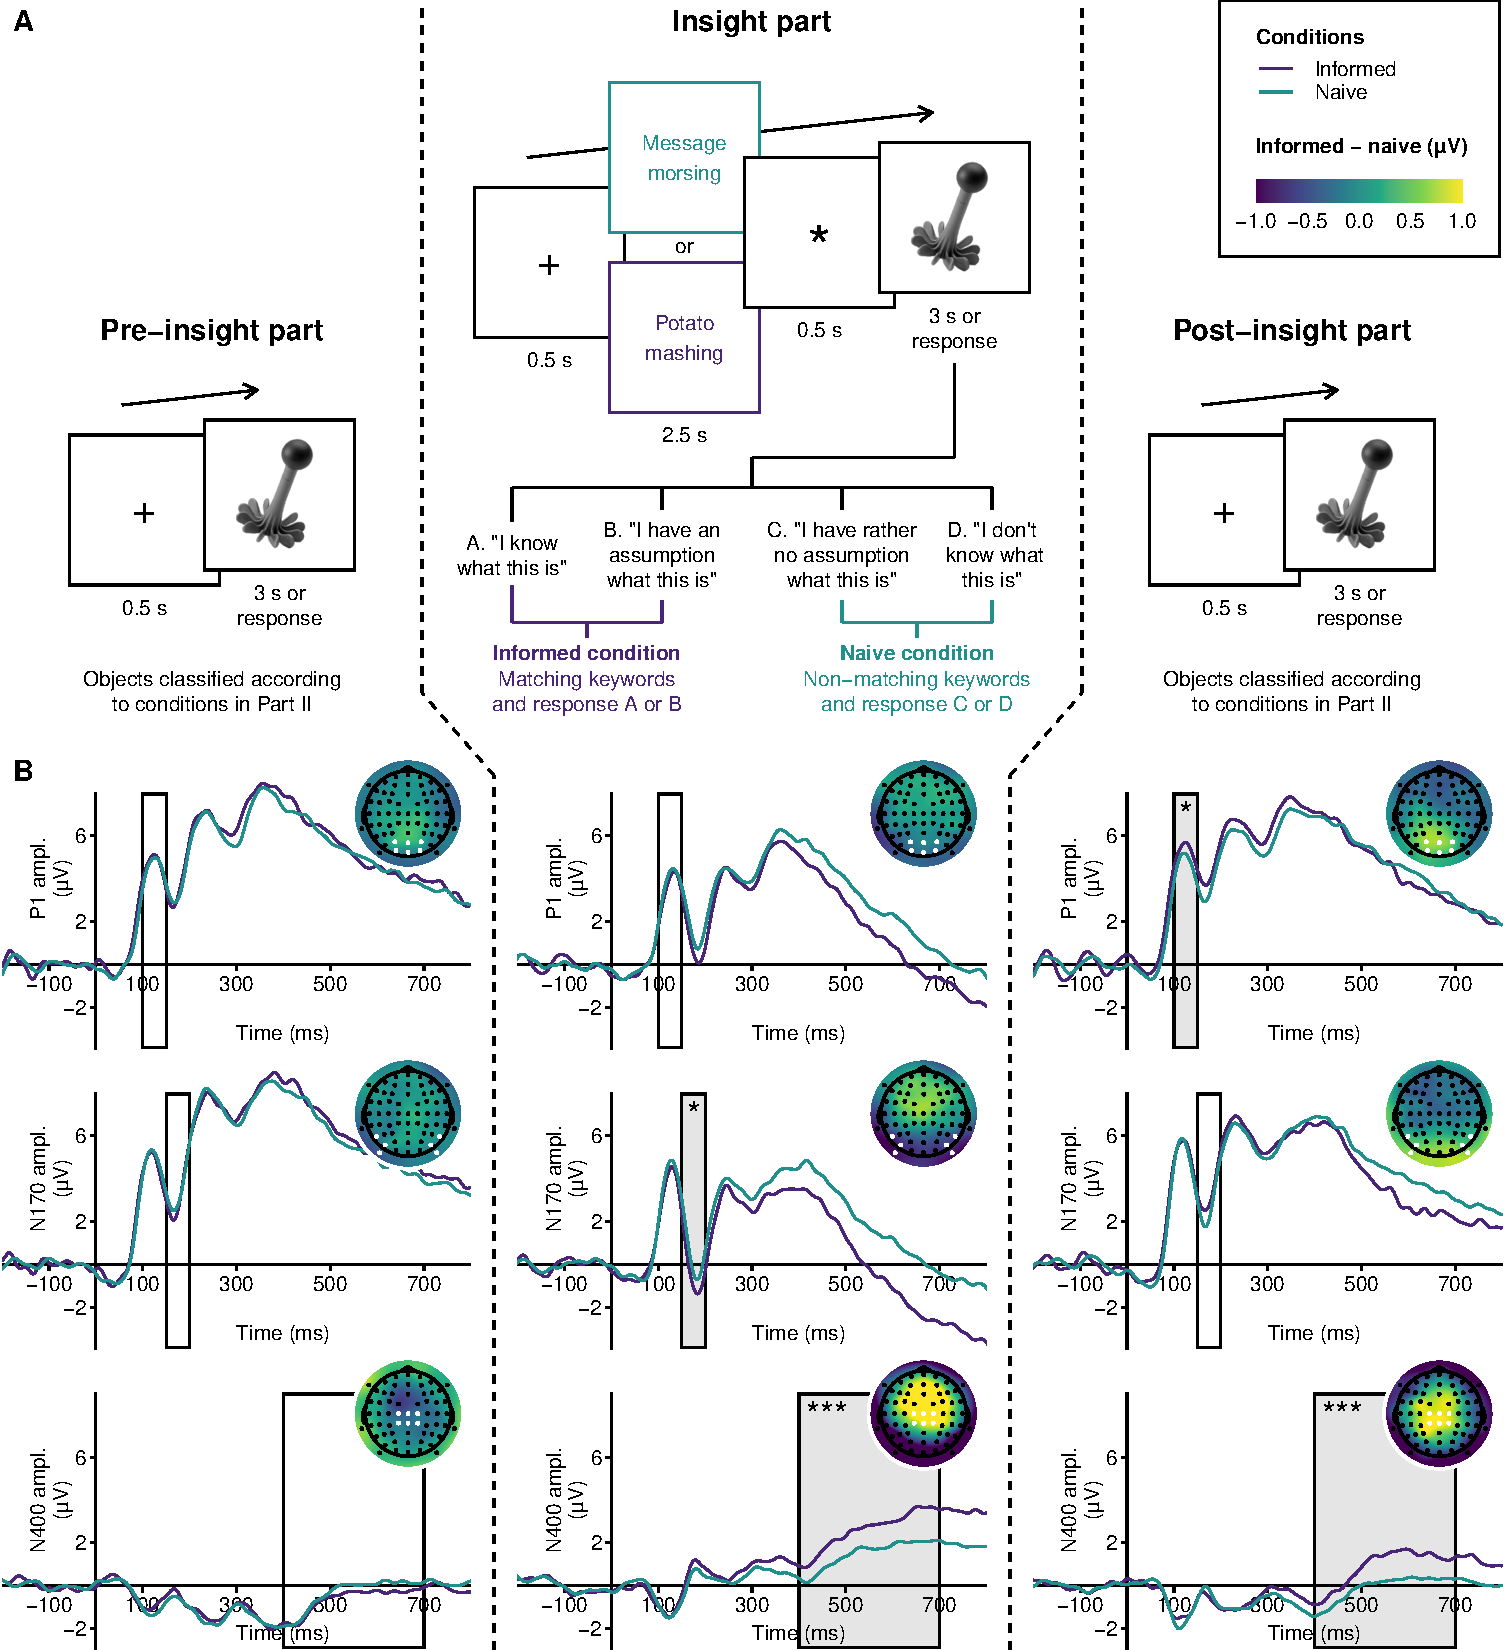
\includegraphics{manuscript_files/figure-latex/exp1-plot-1} 

}

\caption{Procedure and results of Experiment 1. \emph{(A)} In the pre-insight part (Part I) participants were presented with 120 unfamiliar objects and indicated whether they knew what kind of object they were viewing. In the insight part (Part II), half of these objects were presented with matching keywords (in purple color for illustration), leading to semantically informed perception, and the other half with non-matching keywords (in petrol color for illustration), leading to naive perception. In the post-insight part (Part III), the same objects were presented again without the keywords. \emph{(B)} ERP waveforms and scalp topographies separately for objects with semantically informed versus naive perception in Parts I, II, and III. Semantically informed perception was associated with significantly more negative amplitudes in the N1 component in Part II, significantly less negative amplitudes in the N400 component in Parts II and III, and significantly more positive amplitudes in the P1 component in Part III. Ampl. = amplitude.\newline*\emph{p} \textless{} .05. **\emph{p} \textless{} .01. ***\emph{p} \textless{} .001.}\label{fig:exp1-plot}
\end{figure}

In the \emph{insight} part (Part II), only the 120 unfamiliar objects were presented for a second time, now preceded either by matching keywords (leading to semantically informed perception) or by non-matching keywords (leading to naive perception). Each trial consisted of a fixation cross presented for 0.5 s, followed by the presentation of the keywords for 2.5 s. Then, an asterisk was presented in the middle of the screen for another 0.5 s, followed by the presentation of the object until a response was made or until a time out after 3 s. The objects were presented in blocks of 30 trials so that within each block (a) there were 15 objects from each of the two experimental conditions and (b) objects were heterogeneous in terms of their shape, visual complexity, and functional category (e.g.~medical devices, musical instruments).

In the post-insight part (Part III), the unfamiliar objects were presented for a third time with an identical trial structure as in Part I, i.e.~without any keywords. Note that Parts II and III were presented in an interleaved fashion so that after the presentation of one block of 30 objects in Part II (with keywords), participants took a self-timed break and continued with the same block of 30 objects in Part III (without keywords) before moving on to the next block consisting of 30 different objects. They continued like this until all four blocks were completed in both Parts II and III. In total, the experiment consisted of 480 trials (120 familiar objects in Part I and 120 unfamiliar objects in Parts I, II, and III) and took participants approximately 35 minutes to complete.

\hypertarget{eeg-recording-and-preprocessing}{%
\subsubsection{EEG Recording and Preprocessing}\label{eeg-recording-and-preprocessing}}

The continuous EEG was recorded from 62 Ag/AgCl scalp electrodes placed according to the extended 10--20 system (American Electroencephalographic Society, 1991) and referenced online to an external electrode placed on the left mastoid (M1). Two additional external electrodes were placed on the right mastoid (M2) and below the left eye (IO1), respectively. During the recording, electrode impedance was kept below 5 kΩ. An online band-pass filter with a high-pass time-constant of 10 s (0.016 Hz) and a low-pass cutoff frequency of 1,000 Hz was applied before digitizing the signal at a sampling rate of 500 Hz.

Offline, the data were preprocessed using the MNE software (Version 0.21.0; Gramfort et al., 2013) in Python (Version 3.8.5; van Rossum \& Drake, 2009). First, all scalp electrodes were re-referenced to the common average. Next, artifacts resulting from blinks and eye movements were removed using independent component analysis (ICA). The first 15 components were extracted by the FastICA algorithm (Hyvärinen, 1999) after temporarily low-pass filtering the data at 1 Hz. Those components showing substantive correlations with either of two virtual EOG channels (VEOG: IO1 minus Fp1, HEOG: F9 minus F10) were removed automatically using the \emph{find\_bads\_eog} function. After artifact correction, a zero-phase, non-causal FIR filter with a lower pass-band edge at 0.1 Hz (transition bandwidth: 0.1 Hz) and an upper pass-band edge at 30 Hz (transition bandwidth: 7.5 Hz) was applied. Next, the continuous EEG was epoched into segments of 2,000 ms, starting 500 ms before the onset of the visual presentation of each unfamiliar object. The epochs were baseline-corrected by subtracting the average voltage during the 200 ms before stimulus onset. Epochs containing artifacts despite ICA, defined as peak-to-peak amplitudes exceeding 200 µV, were removed from further analysis. This led to the exclusion of an average of 2.4 trials (0.7\%) per participant (range 0 to 24). Single-trial event-related potentials were computed as the mean amplitude across time windows and regions of interests (ROIs) defined a priori, namely 100--150 ms after object onset at electrodes PO3, PO4, POz, O1, O2, and Oz for the P1 component, 150--200 ms after object onset at electrodes P7, P8, PO7, PO8, PO9, and PO10 for the N1 component, and 400--700 ms at electrodes C1, C2, Cz, CP1, CP2, and CPz for the N400 component.

\hypertarget{statistical-analysis}{%
\subsubsection{Statistical Analysis}\label{statistical-analysis}}

First, because we were interested in the effects of knowledge on perceiving \emph{unfamiliar} objects only, we excluded from all furthere analyses those objects which participants classified as being known to them in Part I (i.e.~before any keywords were presented), which led to the exclusion of an average of 7.5 objects per participant (6.3\%). Next, to clearly delineate semantically informed and naive perception, the assignment of all other objects to one of these two conditions for statistical analyses was co-determined by our experimental manipulation (matching versus non-matching keywords in Part II) and the behavioral responses of the participants themselves (Figure 1A). Objects were assigned to the semantically informed condition only if they were presented with matching keywords \emph{and} if participants indicated knowing what the object was or having an assumption. This was the case for an average of 27.0 objects per participant (44.9\% of objects presented with matching keywords). Complementarily, objects were assigned to the naive condition only if they were presented with non-matching keywords \emph{and} if participants indicated not knowing what the object was or having rather no assumption. This was the case for an average of 48.8 objects per participant (81.2\% of objects presented with non-matching keywords). Although the assignment was purely based on the manipulation and responses in Part II, when insight was thought to occurr, the same assignment was used to analyze the data from the other two parts. This allowed us to test on the one hand if the objects from both conditions differed in important aspects even before any keywords were presented (in Part I), and on the other hand if the semantic understanding acquired in Part II had any lasting effects on a subsequent, third presentation of the objects (in Part III).

The event-related potentials in response to objects from both conditions and all three parts were analyzed on the single trial level using linear mixed-effects regression models (Baayen et al., 2008; Frömer et al., 2018). For the purpose of the present study, these models have at least two desirable properties compared to more traditional approaches, such as analyses of variance (ANOVAs) performed on by-participant grand averages. First, they can account simultaneously for the non-independence of data points coming from the same participant or from the same item, whereas the neglect of the item as a random variable in ANOVAs leads to anti-conservative test statistics and strictly does not allow for inferences beyond the stimulus set under study (Bürki et al., 2018; Judd et al., 2012). Second, they can flexibly deal with unbalanced designs in which the number of trials differs across (combinations of) conditions, which is inevitable in designs where the assignment of trials to conditions is (co-)determined by the responses of the participants rather than by the experimental manipulation alone (e.g.~Fröber et al., 2017).

Three separate models were computed predicting P1, N1, and N400 mean amplitudes, respectively. All models included three fixed effects: (a) the part of the experiment, coded as a repeated contrast (i.e.~subtracting Part I from Part II and Part II from Part III, the intercept being the grand mean across all three parts), (b) the condition of the object, coded as a scaled sum contrast (i.e.~subtracting the naive from the semantically informed condition, the intercept being the grand mean across both conditions), and (c) the two-way interaction of part and condition. For details on these and other contrast coding schemes in linear (mixed-effects) models, please refer to (Schad et al., 2020). To determine the random effects structure, we always started with a maximal model containing by-participant and by-item random intercepts and random slopes for all fixed effects (Barr et al., 2013). We then performed a model selection algorithm as proposed by (Matuschek et al., 2017) in order to increase statistical power and avoid overparameterization: Iteratively, each random effects was removed and the resulting, more parsimonious model was compared to the previous, more complex model by means of a likelihood ratio test. Only if the parsimonious model explained the data equally well as the complex model (determined by \emph{p} \textgreater{} .20; Matuschek et al., 2017) did we leave the random effect out, otherwise it was kept in the final model. All models were calculated in R (Version 4.0.2; R Core Team, 2020) using the lme4 package (Version 1.1.23; Bates et al., 2015). The optimizer function \emph{bobyqa} with 2·10\textsuperscript{5} iterations was used for maximum likelihood estimation. The model selection algorithm via likelihood ratio tests was performed using the buildmer package (Version 1.7.1; Voeten, 2020). Finally, to answer our research question of whether or not semantically informed perception had an influence on the ERP components within each part, planned follow-up comparisons were calculated, contrasting the informed against the naive condition within Parts I, II, and III. All \emph{p} values subsequently reported were computed by approximating the relevant denominator degrees of freedom using Satterthwaite's methods as implemented in the lmerTest package (Kuznetsova et al., 2017).

The materials, single trial behavioral and ERP data, and all code for data analysis can be accessed via the Open Science Framework (\href{https://osf.io/myprojects/}{https://osf.io/\ldots/}). To avoid potential misuse, the raw EEG are only made available by the corresponding author upon request.

\hypertarget{results}{%
\subsection{Results}\label{results}}

Single-trial ERPs were analyzed in response to unfamiliar objects before (Part I), while (Part II), and after (Part III) participants obtained relevant semantic information about their function. Only in Part II, half of the objects were preceded by a matching description, fostering semantically informed perception to occur, whereas the other half were preceded by a non-matching description, leading to naive perception of the object. The objects were analyzed according to this manipulation in combination with participants' self-report in Part II (Figure 1A), thus making sure that semantically informed (or naive) perception did indeed occur. The analysis focused on differences between these two conditions in the P1 component (100--150 ms) as an index of lower-level visual perception, in the N1 component (150--200 ms) as index of higher-level visual perception, and in the N400 component (400--700 ms) as an index of semantic processing.

\begin{table}[tbp]

\begin{center}
\begin{threeparttable}

\caption{\label{tab:exp1-table}Results of linear mixed-effects regression models for Experiment 1}

\footnotesize{

\begin{tabular}{lcccccc}
\toprule
 & \multicolumn{2}{c}{\textbf{P1}} & \multicolumn{2}{c}{\textbf{N1}} & \multicolumn{2}{c}{\textbf{N400}} \\
\cmidrule(r){2-3} \cmidrule(r){4-5} \cmidrule(r){6-7}
\textit{Fixed effects} & \textit{F} (\textit{df}) & \textit{p} & \textit{F} (\textit{df}) & \textit{p} & \textit{F} (\textit{df}) & \textit{p}\\
\midrule
Part & 10.82 (2, 24.5) & < .001 & 14.15 (2, 24.9) & < .001 & 33.01 (2, 25.5) & < .001\\
Condition & 0.87 (1, 5302.9) & .351 & 0.89 (1, 114.3) & .349 & 13.09 (1, 24.8) & .001\\
Pt. × con. & 2.40 (2, 4590.9) & .091 & 5.34 (2, 4853.1) & .005 & 11.18 (2, 5030.2) & < .001\\
\textit{Informed $-$  naive} & Est. [95\% CI] & \textit{p} & Est. [95\% CI] & \textit{p} & Est. [95\% CI] & \textit{p}\\ \midrule
Part I & 0.00 [-0.50, 0.49] & .987 & -0.17 [-0.64, 0.30] & .485 & -0.20 [-0.65, 0.26] & .393\\
Part II & -0.15 [-0.65, 0.34] & .550 & -0.66 [-1.14, -0.19] & .006 & 0.93 [0.48, 1.39] & < .001\\
Part III & 0.57 [0.08, 1.07] & .023 & 0.41 [-0.07, 0.88] & .094 & 1.00 [0.55, 1.46] & < .001\\
\bottomrule
\addlinespace
\end{tabular}

}

\begin{tablenotes}[para]
\normalsize{\textit{Note.} Pt. = part, con. = condition, est. = estimate, CI = confidence interval.}
\end{tablenotes}

\end{threeparttable}
\end{center}

\end{table}

Averaged across conditions, P1, N1, and N400 amplitudes differed as a function of the part of the experiment, all \emph{F}s \textgreater{} 10.82, all \emph{p}s \textless{} .001 (Table \ref{tab:exp1-table}). In addition, N400 amplitudes differed between the informed and the naive condition averaged across the three parts of the experiment, \emph{F}NA = NA, \emph{p} = NA. Crucially, the part × condition interaction was significant in the N1 component, \emph{F}(2, 4853.1) = 5.34, \emph{p} = .005, and in the N400 component, \emph{F}(2, 5030.2) = 11.18, \emph{p} \textless{} .001, while also being marginally significant in the P1 component, \emph{F}(2, 4590.9) = 2.40, \emph{p} = .091. To answer our main research question, we decomposed these interactions into the differences between the semantically informed condition and the naive condition within the three different parts of the experiment.

\hypertarget{erps-in-part-i-pre-insight}{%
\subsubsection{ERPs in Part I (Pre-Insight)}\label{erps-in-part-i-pre-insight}}

In Part I, when objects were unfamiliar to the participant and presented without keywords, no differences emerged between the semantically informed and the naive condition in the P1, N1, or N400 component, all \emph{p}s \textgreater{} .393 (Table \ref{tab:exp1-table}, Figure \ref{fig:exp1-plot}B \& C). On the one hand, this was to be expected given that the critical presentation of the keywords (leading to semantically informed vs.~naive perception) had not yet taken place. On the other hand, the absence of reliable differences in Part I can be taken as evidence---with the usual caveats when interpreting null effects---that any subsequent effect of the semantic information in Parts II and III cannot be accounted for by visual differences between the objects in the two conditions. Although the presentation of a matching or non-matching keywords for each object was counterbalanced across participants, the fact that different numbers of objects were assigned to the two conditions based on participants' self report in Part II would have made it possible for such visual differences to emerge as a confounding factor. If they did, however, one would expect to detect these differences even before any keywords were presented, which we have now seen was not the case.

\hypertarget{erps-in-part-ii-insight}{%
\subsubsection{ERPs in Part II (Insight)}\label{erps-in-part-ii-insight}}

In Part II, half of the unfamiliar objects were presented with matching keywords (for forming the semantically informed condition) and the other half were presented with non-matching keywords (for forming the naive condition). When semantic information informed the perception of the object (akin to an insight experience), the amplitude of the N1 component was significantly enlarged (i.e.~more negative), \emph{b} = -0.66 µV, \emph{p} = .006, and the amplitude of the N400 component was significantly reduced (i.e.~less negative), \emph{b} = 0.93 µV, \emph{p} \textless{} .001, compared to when an object was viewed naively without relevant semantic information. As in Part I, there were no reliable differences in the P1 component, \emph{p} = .550.

\hypertarget{erps-in-part-iii-post-insight}{%
\subsubsection{ERPs in Part III (Post-Insight)}\label{erps-in-part-iii-post-insight}}

In Part III, the unfamiliar objects were presented for a third time, again without the keywords (as in Part I), to test whether the semantic information had any lasting effects on the processing of the objects. As in Part II, the N400 component remained significantly reduced during semantically informed as compared to naive perception, \emph{b} = 1.00 µV, \emph{p} \textless{} .001, whereas the early effect in the N1 component did not reoccur, \emph{p} = .094. Instead, we now observed an even earlier modulation in the P1 component, which was significantly enlarged (i.e.~more positive) in response to objects for which semantically informed perception had taken place, \emph{b} = 0.57 µV, \emph{p} = .023.

\hypertarget{discussion}{%
\subsection{Discussion}\label{discussion}}

In Experiment 1, we measured event-related brain potentials from participants viewing unfamiliar objects before (Part I), while (Part II) and after (Part III) they were able to understand what kind of object they saw. To induce this semantically informed perception, half of the objects in Part II were preceded by matching verbal keywords about their typical function or use, whereas the other half were preceded by non-matching keywords, serving as a naive baseline condition.

Participants' semantically informed perception of the objects in Part II was associated with a significantly enlarged N1 component, indicating that the sudden acquisition of knowledge about the object influenced aspects of its higher-level visual processing (Rossion \& Jacques, 2011; Tanaka \& Curran, 2001). The fact that this effect did not reoccur in Part III, when the objects were presented once more without keywords, suggests it being a marker of insight through semantic information that is altering object processing online. In contrast, we also observed a modulation of the N400 component, which was reduced for objects while insight was taking place (in Part II) and remained so when the same objects were presented repeatedly (in Part III). The N400 is most often discussed as an index of increased demands for semantic processing or integration (Kutas \& Federmeier, 2011; Lau et al., 2008; Rabovsky et al., 2018). Its reduction can thus be interpreted as lowered semantic processing demands in response to unfamiliar objects once participants had understood what kind of object they were viewing. Finally, semantically informed perception was also associated with increased amplitudes in the P1 component, but only once the objects were presented for a third time (in Part III), after the critical presentation during which insight had occurred (in Part II). This effect, which replicates previous work on obtaining knowledge about previously unfamiliar images (e.g.~Samaha et al., 2018), may be associated with the newly acquired semantic knowledge exerting an influence on lower-level visual perception, either online or through altered visual representations of the objects for which insight had occurred.

Because of the exploratory nature of the present study and the novelty of the ERP effects observed in Experiment 1, we ran a replication study to assess the robustness of these findings in another samples of participants.

\hypertarget{experiment-2}{%
\section{Experiment 2}\label{experiment-2}}

\hypertarget{methods-1}{%
\subsection{Methods}\label{methods-1}}

\hypertarget{participants-1}{%
\subsubsection{Participants}\label{participants-1}}

Participants for Experiment 2 were 24 German native speakers (15 female, 9 male) with a mean age of 26 years (range 19 to 29) who had not participated in Experiment 1. They had no history of psychological disorder or treatment, were right-handed and reported normal or corrected-to-normal vision. They gave written informed consent before starting the experiment and received a compensation of €8 per hour for participating.

\hypertarget{materials-procedure-and-analysis}{%
\subsubsection{Materials, Procedure, and Analysis}\label{materials-procedure-and-analysis}}

All materials, procedures, EEG-related methods, and statistical analyses were identical to Experiment 1. An average of 7.0 objects per participant (5.8\%) was classified as being known in Part I and excluded from all further analyses. Based on participants' responses in Part II, an average of 26.4 objects were assigned to the semantically informed condition (44.0\% of objects presented with matching keywords) and an average of 49.2 objects were assigned to the naive condition (82.0\% of objects presented with a non-matching description). Automatic rejection of EEG epochs containing artifacts led to the exclusion of 11.0 trials per participant (3.0\%, range 0 to 85).

\hypertarget{results-1}{%
\subsection{Results}\label{results-1}}

\begin{table}[tbp]

\begin{center}
\begin{threeparttable}

\caption{\label{tab:exp2-table}Results of linear mixed-effects regression models for Experiment 2}

\footnotesize{

\begin{tabular}{lcccccc}
\toprule
 & \multicolumn{2}{c}{\textbf{P1}} & \multicolumn{2}{c}{\textbf{N1}} & \multicolumn{2}{c}{\textbf{N400}} \\
\cmidrule(r){2-3} \cmidrule(r){4-5} \cmidrule(r){6-7}
\textit{Fixed effects} & \textit{F} (\textit{df}) & \textit{p} & \textit{F} (\textit{df}) & \textit{p} & \textit{F} (\textit{df}) & \textit{p}\\
\midrule
Part & 18.14 (2, 5151.1) & < .001 & 16.39 (2, 25.0) & < .001 & 70.58 (2, 25.2) & < .001\\
Condition & 0.03 (1, 5272.5) & .853 & 1.23 (1, 5218.6) & .267 & 18.66 (1, 5207.5) & < .001\\
Pt. × con. & 3.74 (2, 5151.2) & .024 & 1.34 (2, 4736.8) & .263 & 8.07 (2, 4637.6) & < .001\\
\textit{Informed $-$  naive} & Est. [95\% CI] & \textit{p} & Est. [95\% CI] & \textit{p} & Est. [95\% CI] & \textit{p}\\ \midrule
Part I & -0.17 [-0.72, 0.38] & .552 & -0.04 [-0.53, 0.45] & .864 & 0.02 [-0.44, 0.48] & .936\\
Part II & -0.49 [-1.04, 0.07] & .084 & -0.50 [-0.99, 0.00] & .050 & 1.31 [0.86, 1.77] & < .001\\
Part III & 0.56 [0.01, 1.11] & .048 & 0.04 [-0.45, 0.54] & .865 & 0.45 [-0.01, 0.91] & .055\\
\bottomrule
\addlinespace
\end{tabular}

}

\begin{tablenotes}[para]
\normalsize{\textit{Note.} Pt. = part, con. = condition, est. = estimate, CI = confidence interval.}
\end{tablenotes}

\end{threeparttable}
\end{center}

\end{table}

As in Experiment 1, P1, N1, and N400 amplitudes differed between the three different parts of the experiments, all \emph{F}s \textgreater{} 16.39, all \emph{p}s \textless{} .001 (Table \ref{tab:exp2-table}). Also as in Experiment 1, N400 amplitudes differed between the informed and the naive condition averaged across parts, \emph{F}NA = NA, \emph{p} NA. The part × condition interaction was significant in the P1 component, \emph{F}(2, 5151.2) = 3.74, \emph{p} = .024, and in the N400 component, \emph{F}(2, 4637.6) = 8.07, \emph{p} \textless{} .001, but not in the N1 component, \emph{F}(2, 4736.8) = 1.34, \emph{p} = .263.



\begin{figure}

{\centering 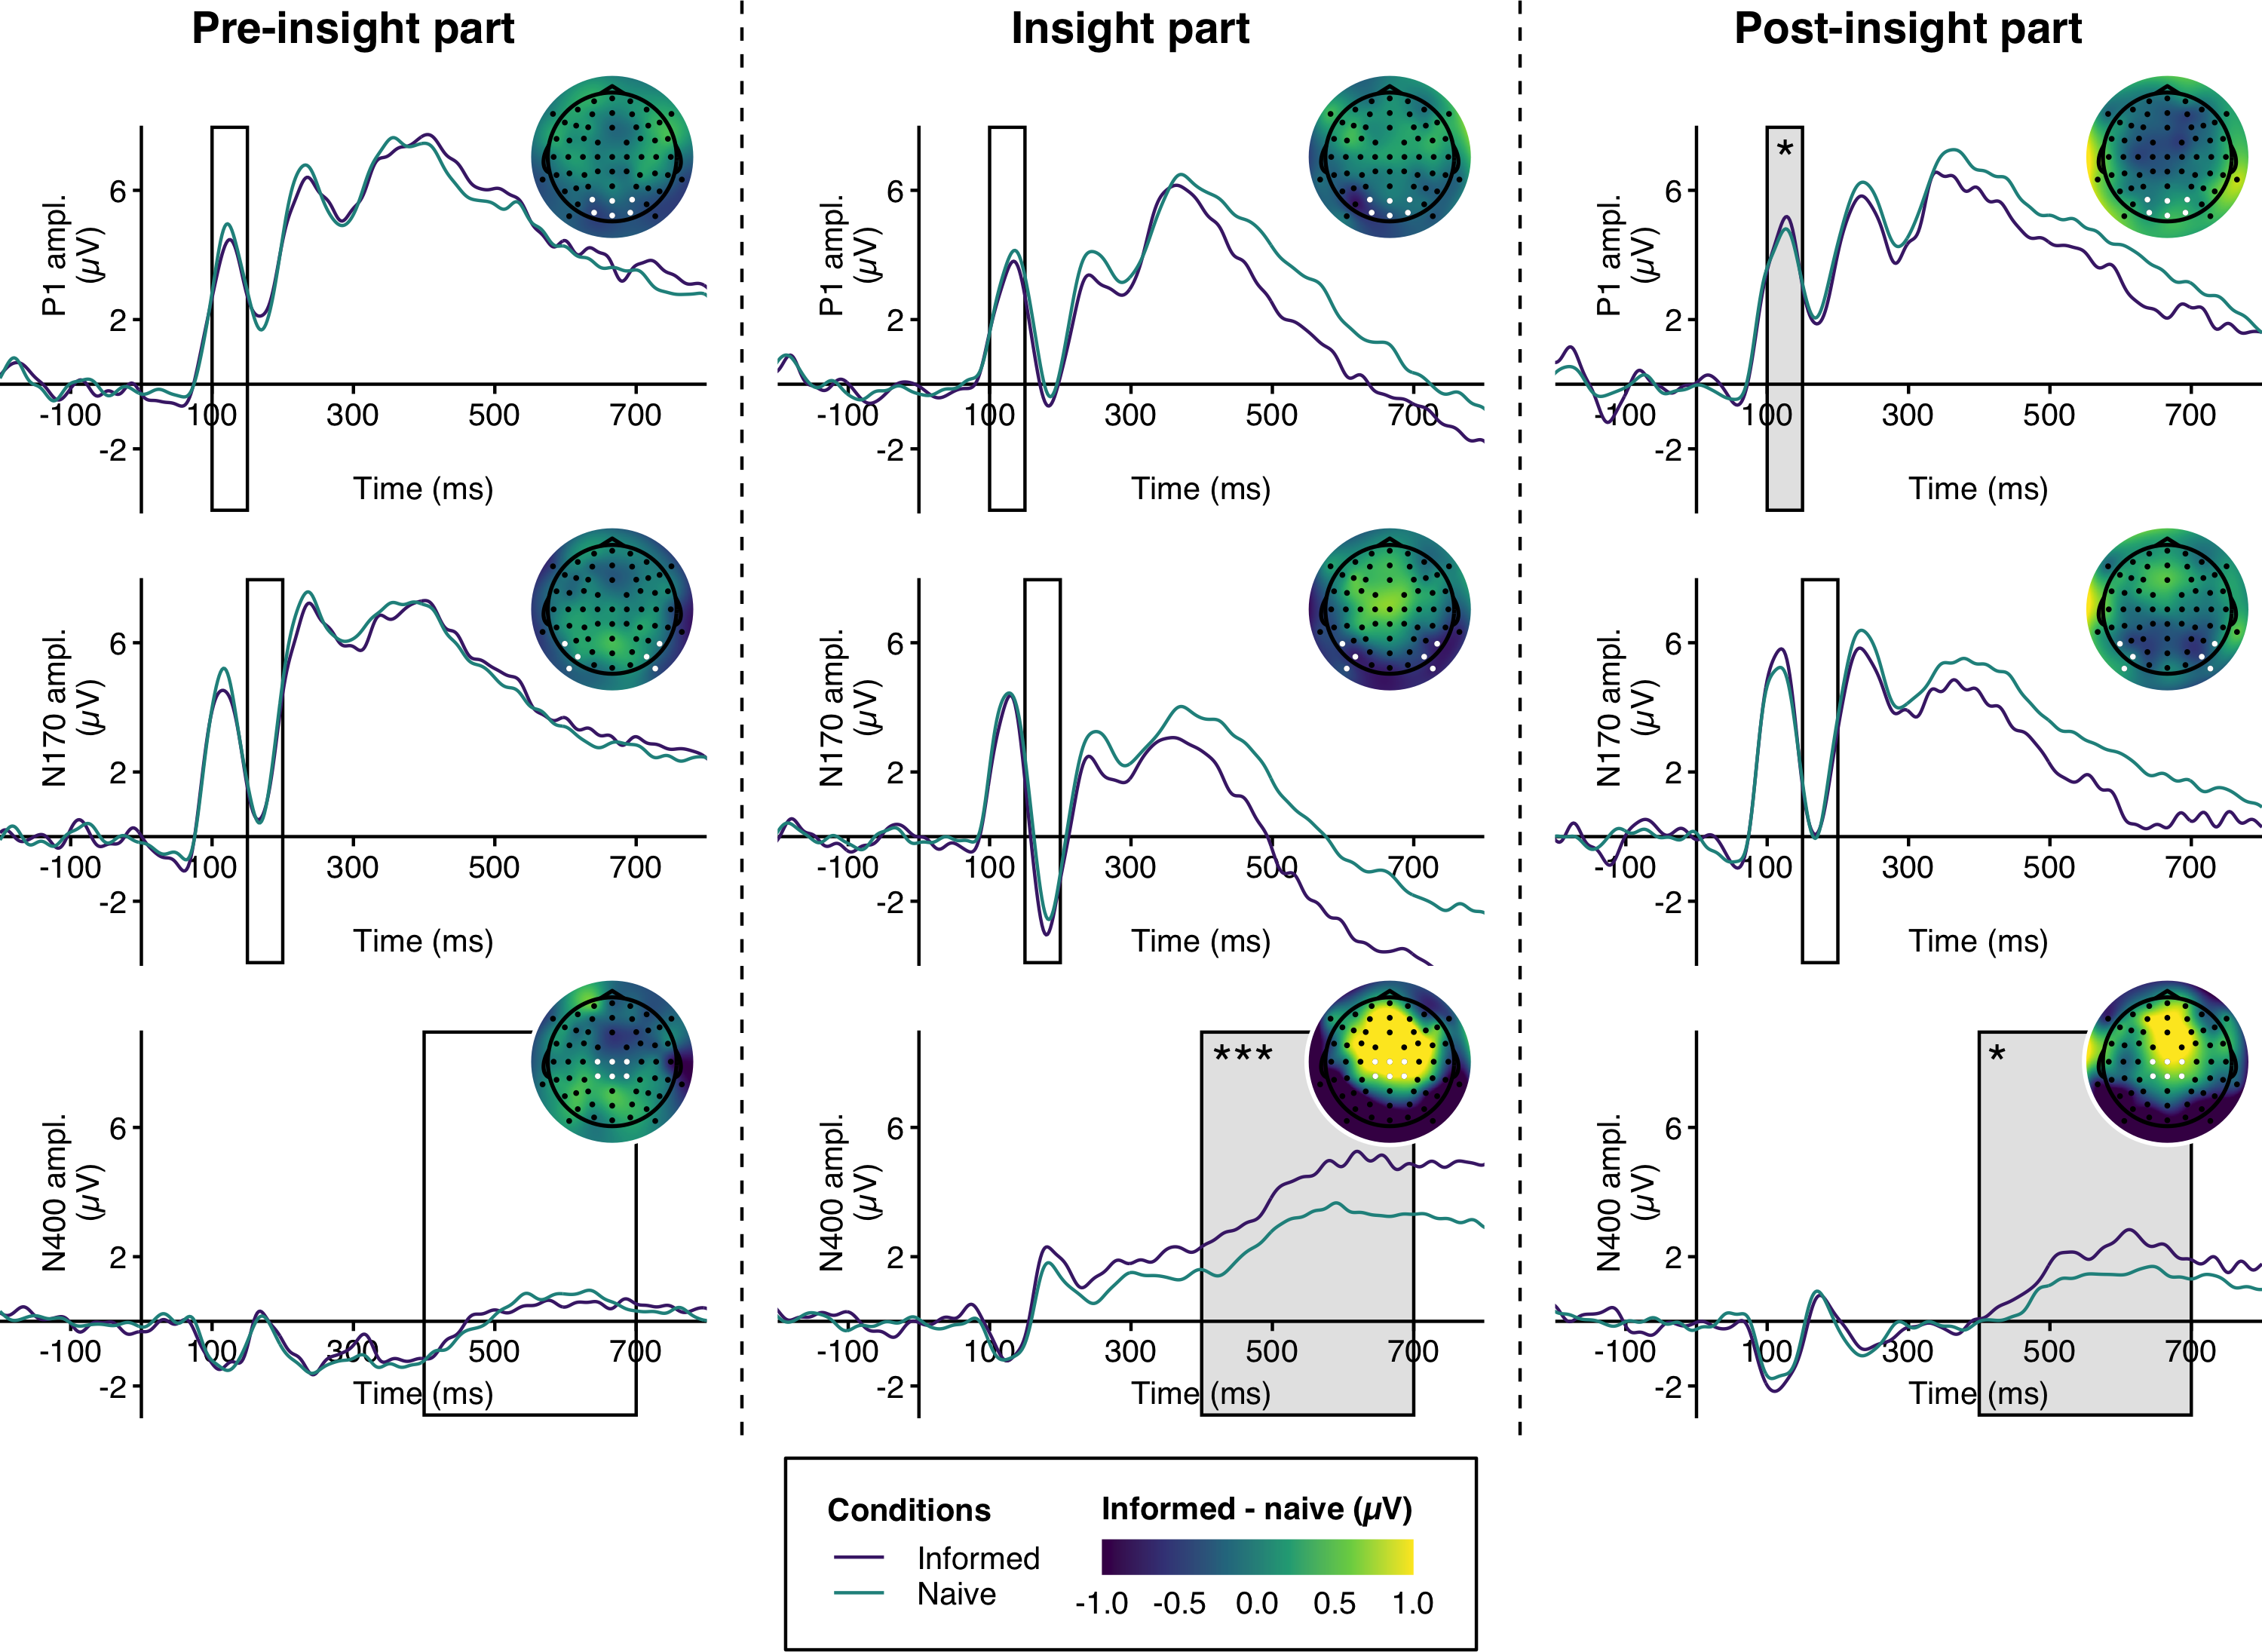
\includegraphics{manuscript_files/figure-latex/exp2-plot-1} 

}

\caption{Results of Experiment 2. ERP waveforms and scalp topographies separately for objects for which participants experienced semantically informed versus naive perception in Parts I, II, and III. In a direct replication of Experiment 1, the effect of semantic information on the N400 component in Parts II and III and on the P1 component in Part III remained statistically significant, while the effect on the N1 component in Part II remained only marginally significant. Ampl. = amplitude.\newline*\emph{p} \textless{} .05. ***\emph{p} \textless{} .001.}\label{fig:exp2-plot}
\end{figure}

\hypertarget{erps-in-part-i-pre-insight-1}{%
\subsubsection{ERPs in Part I (Pre-Insight)}\label{erps-in-part-i-pre-insight-1}}

As in Experiment 1, no differences between objects in the semantically informed and the naive condition emerged in the P1, N1, or N400 component, all \emph{p}s \textgreater{} .552 (Table \ref{tab:exp2-table}, Figure \ref{fig:exp2-plot}).

\hypertarget{erps-in-part-ii-insight-1}{%
\subsubsection{ERPs in Part II (Insight)}\label{erps-in-part-ii-insight-1}}

As in Experiment 1, semantically informed as compared to naive perception (induced by matching versus non-matching keywords) was associated with a (marginally) significant enhancement of the N1 component, \emph{b} = -0.50 µV, \emph{p} = .050, and a significant reduction of the N400 component, \emph{b} = 0.93 µV, \emph{p} \textless{} .001.

\hypertarget{erps-in-part-iii-post-insight-1}{%
\subsubsection{ERPs in Part III (Post-Insight)}\label{erps-in-part-iii-post-insight-1}}

As in Experiment 1, the presentation of the same unfamiliar objects for a third time (without keywords, as in Part I) led to significantly larger amplitudes in the P1 component in response to objects for which semantically informed perception had occurred, \emph{b} = 0.56 µV, \emph{p} = .048. Also, N400 amplitudes in response to these objects remained significantly reduced, \emph{b} = 0.45 µV, \emph{p} = .055.

\hypertarget{joint-analysis-of-experiments-1-and-2}{%
\subsubsection{Joint Analysis of Experiments 1 and 2}\label{joint-analysis-of-experiments-1-and-2}}

In an attempt to maximize statistical power, we combined the ERP data sets from Experiments 1 and 2. This allowed us to determine (a) if the above effects---including the marginally significant ones---were reliable when tested in a larger sample, and (b) if there were significant differences in the ERP amplitudes between Experiments 1 and 2. Methods for statistical analysis were kept unchanged apart from the addition of a new factor denoting the experiment, coded as a scaled sum contrast (i.e.~subtracting Experiment 1 from Experiment 2, the intercept being the grand mean across both experiments; Schad et al., 2020). This factor and its possible interactions with part, condition, and part × condition were included in the linear mixed-effects regression models as fixed effects and as potential by-item random slopes. They were not included as by-participant random slopes since different participants took part in Experiments 1 and 2. Note that, as above, random effects were eventually included only if their omission led to a significant decline in model fit (Matuschek et al., 2017; Voeten, 2020).

\begin{table}[tbp]

\begin{center}
\begin{threeparttable}

\caption{\label{tab:joint-table}Results of linear mixed-effects regression models for Experiments 1 and 2 combined}

\footnotesize{

\begin{tabular}{lcccccc}
\toprule
 & \multicolumn{2}{c}{\textbf{P1}} & \multicolumn{2}{c}{\textbf{N1}} & \multicolumn{2}{c}{\textbf{N400}} \\
\cmidrule(r){2-3} \cmidrule(r){4-5} \cmidrule(r){6-7}
\textit{Fixed effects} & \textit{F} (\textit{df}) & \textit{p} & \textit{F} (\textit{df}) & \textit{p} & \textit{F} (\textit{df}) & \textit{p}\\
\midrule
Part & 12.38 (2, 49.0) & < .001 & 29.90 (2, 50.0) & < .001 & 95.34 (2, 50.6) & < .001\\
Condition & 0.35 (1, 10560.3) & .552 & 1.65 (1, 125.3) & .202 & 38.72 (1, 10518.8) & < .001\\
Experiment & 0.35 (1, 48.2) & .555 & 2.38 (1, 48.1) & .129 & 4.75 (1, 48.4) & .034\\
Pt. × con. & 4.02 (2, 9042.4) & .018 & 5.60 (2, 9877.5) & .004 & 15.73 (2, 10010.1) & < .001\\
Pt. × exp. & 0.03 (2, 49.0) & .971 & 0.55 (2, 50.0) & .581 & 2.58 (2, 50.6) & .085\\
Ins. × exp. & 0.62 (1, 10536.2) & .432 & 0.04 (1, 10332.1) & .838 & 0.03 (1, 10574.9) & .865\\
Pt. × con. × exp. & 0.03 (2, 9042.9) & .972 & 0.62 (2, 9877.8) & .537 & 2.65 (2, 10010.4) & .070\\
\textit{Informed $-$  naive} & Est. [95\% CI] & \textit{p} & Est. [95\% CI] & \textit{p} & Est. [95\% CI] & \textit{p}\\ \midrule
Part I & -0.07 [-0.44, 0.30] & .699 & -0.10 [-0.44, 0.24] & .568 & -0.10 [-0.41, 0.20] & .507\\
Part II & -0.22 [-0.59, 0.15] & .248 & -0.56 [-0.90, -0.21] & .002 & 1.09 [0.79, 1.39] & < .001\\
Part III & 0.49 [0.12, 0.86] & .010 & 0.25 [-0.10, 0.59] & .158 & 0.72 [0.41, 1.02] & < .001\\
\bottomrule
\addlinespace
\end{tabular}

}

\begin{tablenotes}[para]
\normalsize{\textit{Note.} Pt. = part, con. = condition, exp. = experiment, est. = estimate, CI = confidence interval.}
\end{tablenotes}

\end{threeparttable}
\end{center}

\end{table}

As shown in Table \ref{tab:joint-table}, the main effect of the part of the experiment was significant in the P1, N1, and N400 component, all \emph{F}s \textgreater{} 12.38, all \emph{p}s \textless{} .001, as was the main effect of condition in the N400, \emph{F}NA = NA, \emph{p} NA. Furthermore, the part × condition interaction was now observed reliably in all three components, all \emph{F}s \textgreater{} 4.02, all \emph{p}s \textless{} .018. While there was a main effect of experiment in the N400, \emph{F}(1, 48.4) = 4.75, \emph{p} = .034, the absence of any significant interactions of experiment with part or condition indicated that the effects of our experimental manipulations did not differ between Experiments 1 and 2.

Based on the part × condition interaction, we again computed follow-up comparisons between the semantically inforemd and the naive condition within each part, now collapsed across the data from both experiments. This confirmed the absence of any reliable differences between the two conditions in Part I, all \emph{p}s \textgreater{} .507, the significant enhancement of the N1 component in Part II, while the semantic information was obtained, \emph{b} = -0.56 µV, \emph{p} = .002, the significant reduction of the N400 component in Part II, while the semantic information was obtained, \emph{b} = 1.09 µV, \emph{p} \textless{} .001, and Part III, after the information had been obtained, \emph{b} = 0.72 µV, \emph{p} = \textless{} .001, as well as the significant enhancement of the P1 component in Part III, after the information had been obtained, \emph{b} = 0.49 µV, \emph{p} = .010.

\hypertarget{control-analysis}{%
\subsubsection{Control Analysis}\label{control-analysis}}

One may raise concerns whether the modulation of the N1 component in Part II genuinely reflects the semantically informed perception of the objects in the respective condition, or---as an alternative explanation---whether it could be driven by the objects in the other, semantically naive condition. Remember that these objects were preceded by non-matching keywords which were picked so that they could not be related to the object's visual features and their configuration. Thus, the modulation of the ERP components in Part II may reflect a mismatch response to those objects---reflecting, for example, the fact that the visual features of the object shown in Figure \ref{fig:exp1-plot}A cannot be reconciled with the function of morsing messages. To preclude this alternative explanation, we repeated the analysis above using a different baseline against which the objects in the semantically informed condition were contrasted. Instead of the naive condition (where objects were presented with non-matching descriptions), we now used those objects which were preceded by matching descriptions (as in the informed condition), but which were excluded from the main analysis because participants indicated behaviorally that they did not understand the object they were seeing. Across both experiments, this was the case for 49.6\% of objects presented with matching descriptions as compared to 44.4\% of objects which did indeed lead to semantically informed perception.\footnote{Note that the remaining objects to make it up to 100\% were excluded as not being unfamiliar in Part I of the experiment (see Statistical Analysis)} Just as above, this control analysis revealed a robust N1 effect in Part II, \emph{b} = -0.99 µV, \emph{p} \textless{} .001. Thus, this enhanced negativity seems to be a genuine marker of semantically informed perception, no matter if compared to objects presented with misleading keywords or compared to objects presented with accurate keywords on which participants failed to capitalize. Note that the reduction of the N400 component in Part II also remained robust in this control analysis, \emph{b} = 1.19 µV, \emph{p} \textless{} .001.

\hypertarget{discussion-1}{%
\subsection{Discussion}\label{discussion-1}}

Experiment 2, which was a direct replication of Experiment 1, confirmed the effects of obtaining semantic information about previously unfamiliar objects on ERPs associated with lower-level visual perception (P1), higher-level visual perception (N1), and semantic processing (N400). While the enhancement of the N1 component, being more negative for semantically informed as compared to naive perception, was present only during the critical presentation of the objects with their respective keywords (in Part II), the enhancement of the P1, being more positive in response to these same objects, emerged only after the information had been obtained and the objects were presented again (in Part III). This indicates a modulation of different stages of visual object perception through semantic knowledge, while and after an understanding of the object has been obtained. Finally, a sustained reduction of the N400 component in response to objects for which participants experienced semantically informed perception may reflect lowered semantic processing demands compared to unfamiliar objects which participants did not yet understand.

\hypertarget{general-discussion}{%
\section{General Discussion}\label{general-discussion}}

General discussion section goes here.

\newpage

\hypertarget{references}{%
\section{References}\label{references}}

\setlength{\parindent}{-0.5in}

\hypertarget{refs}{}
\begin{cslreferences}
\leavevmode\hypertarget{ref-abdelrahman2008}{}%
Abdel Rahman, R., \& Sommer, W. (2008). Seeing what we know and understand: How knowledge shapes perception. \emph{Psychonomic Bulletin \& Review}, \emph{15}(6), 1055--1063. \url{https://doi.org/10.3758/PBR.15.6.1055}

\leavevmode\hypertarget{ref-americanelectroencephalographicsociety1991}{}%
American Electroencephalographic Society. (1991). American Electroencephalographic Society guidelines for standard electrode position nomenclature. \emph{Journal of Clinical Neurophysiology}, \emph{8}(2), 200--202.

\leavevmode\hypertarget{ref-baayen2008}{}%
Baayen, R. H., Davidson, D. J., \& Bates, D. M. (2008). Mixed-effects modeling with crossed random effects for subjects and items. \emph{Journal of Memory and Language}, \emph{59}(4), 390--412. \url{https://doi.org/10.1016/j.jml.2007.12.005}

\leavevmode\hypertarget{ref-barr2013}{}%
Barr, D. J., Levy, R., Scheepers, C., \& Tily, H. J. (2013). Random effects structure for confirmatory hypothesis testing: Keep it maximal. \emph{Journal of Memory and Language}, \emph{68}(3), 255--278. \url{https://doi.org/10.1016/j.jml.2012.11.001}

\leavevmode\hypertarget{ref-R-lme4}{}%
Bates, D., Mächler, M., Bolker, B., \& Walker, S. (2015). Fitting linear mixed-effects models using lme4. \emph{Journal of Statistical Software}, \emph{67}(1), 1--48. \url{https://doi.org/10.18637/jss.v067.i01}

\leavevmode\hypertarget{ref-buxfcrki2018}{}%
Bürki, A., Frossard, J., \& Renaud, O. (2018). Accounting for stimulus and participant effects in event-related potential analyses to increase the replicability of studies. \emph{Journal of Neuroscience Methods}, \emph{309}, 218--227. \url{https://doi.org/10.1016/j.jneumeth.2018.09.016}

\leavevmode\hypertarget{ref-firestone2016}{}%
Firestone, C., \& Scholl, B. J. (2016). Cognition does not affect perception: Evaluating the evidence for ``top-down'' effects. \emph{Behavioral and Brain Sciences}, \emph{39}. \url{https://doi.org/10.1017/S0140525X15000965}

\leavevmode\hypertarget{ref-fruxf6ber2017}{}%
Fröber, K., Stürmer, B., Frömer, R., \& Dreisbach, G. (2017). The role of affective evaluation in conflict adaptation: An LRP study. \emph{Brain and Cognition}, \emph{116}, 9--16. \url{https://doi.org/10.1016/j.bandc.2017.05.003}

\leavevmode\hypertarget{ref-fruxf6mer2018}{}%
Frömer, R., Maier, M., \& Abdel Rahman, R. (2018). Group-level EEG-processing pipeline for flexible single trial-based analyses including linear mixed models. \emph{Frontiers in Neuroscience}, \emph{12}. \url{https://doi.org/10.3389/fnins.2018.00048}

\leavevmode\hypertarget{ref-gauthier2003}{}%
Gauthier, I., James, T. W., Curby, K. M., \& Tarr, M. J. (2003). The influence of conceptual knowledge on visual discrimination. \emph{Cognitive Neuropsychology}, \emph{20}(3-6), 507--523. \url{https://doi.org/10.1080/02643290244000275}

\leavevmode\hypertarget{ref-gramfort2013}{}%
Gramfort, A., Luessi, M., Larson, E., Engemann, D. A., Strohmeier, D., Brodbeck, C., Goj, R., Jas, M., Brooks, T., Parkkonen, L., \& al. (2013). MEG and EEG data analysis with MNE-Python. \emph{Frontiers in Neuroscience}, \emph{7}. \url{https://doi.org/10.3389/fnins.2013.00267}

\leavevmode\hypertarget{ref-gratton2009}{}%
Gratton, C., Evans, K. M., \& Federmeier, K. D. (2009). See what I mean? An ERP study of the effect of background knowledge on novel object processing. \emph{Memory \& Cognition}, \emph{37}(3), 277--291. \url{https://doi.org/10.3758/MC.37.3.277}

\leavevmode\hypertarget{ref-holmes2012}{}%
Holmes, K. J., \& Wolff, P. (2012). Does categorical perception in the left hemisphere depend on language? \emph{Journal of Experimental Psychology. General}, \emph{141}(3), 439--443. \url{https://doi.org/10.1037/a0027289}

\leavevmode\hypertarget{ref-hyvuxe4rinen1999}{}%
Hyvärinen, A. (1999). Fast and robust fixed-point algorithms for independent component analysis. \emph{IEEE Transactions on Neural Networks}, \emph{10}(3), 626--634. \url{https://doi.org/10.1109/72.761722}

\leavevmode\hypertarget{ref-judd2012}{}%
Judd, C. M., Westfall, J., \& Kenny, D. A. (2012). Treating stimuli as a random factor in social psychology: A new and comprehensive solution to a pervasive but largely ignored problem. \emph{Journal of Personality and Social Psychology}, \emph{103}(1), 54--69. \url{https://doi.org/10.1037/a0028347}

\leavevmode\hypertarget{ref-kutas2011}{}%
Kutas, M., \& Federmeier, K. D. (2011). Thirty years and counting: Finding meaning in the N400 component of the event-related brain potential (ERP). \emph{Annual Review of Psychology}, \emph{62}, 621--647. \url{https://doi.org/10.1146/annurev.psych.093008.131123}

\leavevmode\hypertarget{ref-R-lmerTest}{}%
Kuznetsova, A., Brockhoff, P. B., \& Christensen, R. H. B. (2017). lmerTest package: Tests in linear mixed effects models. \emph{Journal of Statistical Software}, \emph{82}(13), 1--26. \url{https://doi.org/10.18637/jss.v082.i13}

\leavevmode\hypertarget{ref-lau2008}{}%
Lau, E. F., Phillips, C., \& Poeppel, D. (2008). A cortical network for semantics: (De)constructing the N400. \emph{Nature Reviews Neuroscience}, \emph{9}(12), 920--933. \url{https://doi.org/10.1038/nrn2532}

\leavevmode\hypertarget{ref-maier2014}{}%
Maier, M., Glage, P., Hohlfeld, A., \& Abdel Rahman, R. (2014). Does the semantic content of verbal categories influence categorical perception? An ERP study. \emph{Brain and Cognition}, \emph{91}, 1--10. \url{https://doi.org/10.1016/j.bandc.2014.07.008}

\leavevmode\hypertarget{ref-maier2019}{}%
Maier, M., \& Rahman, R. A. (2019). No matter how: Top-down effects of verbal and semantic category knowledge on early visual perception. \emph{Cognitive, Affective, \& Behavioral Neuroscience}, \emph{19}(4), 859--876. \url{https://doi.org/10.3758/s13415-018-00679-8}

\leavevmode\hypertarget{ref-matuschek2017}{}%
Matuschek, H., Kliegl, R., Vasishth, S., Baayen, H., \& Bates, D. (2017). Balancing Type I error and power in linear mixed models. \emph{Journal of Memory and Language}, \emph{94}, 305--315. \url{https://doi.org/10.1016/j.jml.2017.01.001}

\leavevmode\hypertarget{ref-oldfield1971}{}%
Oldfield, R. C. (1971). The assessment and analysis of handedness: The Edinburgh inventory. \emph{Neuropsychologia}, \emph{9}(1), 97--113. \url{https://doi.org/10.1016/0028-3932(71)90067-4}

\leavevmode\hypertarget{ref-rabovsky2018}{}%
Rabovsky, M., Hansen, S. S., \& McClelland, J. L. (2018). Modelling the N400 brain potential as change in a probabilistic representation of meaning. \emph{Nature Human Behaviour}, \emph{2}(9), 693--705. \url{https://doi.org/10.1038/s41562-018-0406-4}

\leavevmode\hypertarget{ref-R-base}{}%
R Core Team. (2020). \emph{R: A language and environment for statistical computing}. R Foundation for Statistical Computing. \url{https://www.R-project.org/}

\leavevmode\hypertarget{ref-rossion2002}{}%
Rossion, B., Gauthier, I., Goffaux, V., Tarr, M. J., \& Crommelinck, M. (2002). Expertise training with novel objects leads to left-lateralized facelike electrophysiological responses. \emph{Psychological Science}. \url{https://journals.sagepub.com/doi/10.1111/1467-9280.00446}

\leavevmode\hypertarget{ref-rossion2011}{}%
Rossion, B., \& Jacques, C. (2011). The N170: Understanding the time course of face perception in the human brain. In E. S. Kappenman \& S. J. Luck (Eds.), \emph{The Oxford handbook of event-related potential components} (pp. 115--142). Oxford University Press. \url{https://doi.org/10.1093/oxfordhb/9780195374148.001.0001}

\leavevmode\hypertarget{ref-rossion2004}{}%
Rossion, B., Kung, C.-C., \& Tarr, M. J. (2004). Visual expertise with nonface objects leads to competition with the early perceptual processing of faces in the human occipitotemporal cortex. \emph{Proceedings of the National Academy of Sciences of the United States of America}, \emph{101}(40), 14521--14526. \url{https://doi.org/10.1073/pnas.0405613101}

\leavevmode\hypertarget{ref-samaha2018}{}%
Samaha, J., Boutonnet, B., Postle, B. R., \& Lupyan, G. (2018). Effects of meaningfulness on perception: Alpha-band oscillations carry perceptual expectations and influence early visual responses. \emph{Scientific Reports}, \emph{8}(1), 1--14. \url{https://doi.org/10.1038/s41598-018-25093-5}

\leavevmode\hypertarget{ref-schad2020}{}%
Schad, D. J., Vasishth, S., Hohenstein, S., \& Kliegl, R. (2020). How to capitalize on a priori contrasts in linear (mixed) models: A tutorial. \emph{Journal of Memory and Language}, \emph{110}, 104038. \url{https://doi.org/10.1016/j.jml.2019.104038}

\leavevmode\hypertarget{ref-tanaka2001}{}%
Tanaka, J. W., \& Curran, T. (2001). A neural basis for expert object recognition. \emph{Psychological Science}, \emph{12}(1), 43--47. \url{https://doi.org/10.1111/1467-9280.00308}

\leavevmode\hypertarget{ref-vanrossum2009}{}%
van Rossum, G., \& Drake, F. L. (2009). \emph{Python 3 reference manual}. CreateSpace.

\leavevmode\hypertarget{ref-R-buildmer}{}%
Voeten, C. C. (2020). \emph{buildmer: Stepwise elimination and term reordering for mixed-effects regression}. \url{https://CRAN.R-project.org/package=buildmer}

\leavevmode\hypertarget{ref-weller2019}{}%
Weller, P. D., Rabovsky, M., \& Abdel Rahman, R. (2019). Semantic knowledge enhances conscious awareness of visual objects. \emph{Journal of Cognitive Neuroscience}, \emph{31}(8), 1216--1226. \url{https://doi.org/10.1162/jocn_a_01404}
\end{cslreferences}


\end{document}
